\documentclass{report}
\usepackage[utf8]{inputenc}
\usepackage{lineno}
\linenumbers

\usepackage{hyperref}
\hypersetup{
    colorlinks,
    citecolor=blue,
    filecolor=black,
    linkcolor=black,
    urlcolor=black
}




\title{Privacy Oriented Data Analysis}
\author{Muhammad Umer Altaf }
\date{October 2017}

\usepackage{natbib}
\usepackage{graphicx}
\newcommand\Chapter[2]{
  \chapter[#1: {\itshape#2}]{#1\\[2ex]\Large\itshape#2}
}





\begin{document}

\maketitle
\setcounter{tocdepth}{1}
\tableofcontents

\chapter{Introduction}


\textit{``The choice for mankind lies between freedom and happiness and for the great bulk of mankind, happiness is better."}

{\raggedleft -- George Orwell in `1984'\quad\par}




\chapter{Privacy-oriented Data Analysis in Distributed and Hybrid Environments}{Background Study}
\section{Introduction}
\paragraph{}
Systems that guarantee secure communication have been in use for a long time, but Public Clouds suffer from very basic trust issues. Sensitive data like medical or financial records have tough safety guidelines and cannot be processed on offshore third party servers. The advent of public cloud holds tremendous advantages in terms of scalability and elasticity, especially if augmented by in-house infrastructure (Hybrid Cloud). In this chapter we will list some of existing frameworks that try to support privacy oriented analysis while being applicable in hybrid clouds or distributed environments.
\paragraph{}
The ideal of Privacy in Data Analysis can be traced back to Dalenius 1977’s \cite{dalenius1977} rule, that no such information about a single person can be derived from a database that cannot be learned without access to the database. This simply means that in a secure privacy controlled analysis, the results can never lead to private data.
\paragraph{}
Organizations are hungry for insights from Big Data. Online advertisement agencies and social media networks are already using these insights to drive profits by serving targeted advertisements. Retailers use these insights to identify patterns in markets and sales. Most of currently prevalent applications care very less about individual privacy because in most cases the individual has voluntarily forfeited the right to privacy (see Terms and Conditions on Facebook Sign-up).
\paragraph{}
There are however some applications where this privacy of individual holds the prime objective yet the analytic potential of data as whole is also very great. For example processing large data of psoriasis patients may bring useful insights about the disease, but if some health insurance company is able to identify patients and refuse coverage then it can be both, legally and ethically wrong. 
Below we discuss some of the identified formalization of privacy problems in Big Data context and some proposed solutions.

\section{Methodologies for Private Data Analysis}
\paragraph{}
The traditional methodology for privacy protection has been mandated access control. This is the protection of data resources via set policy controls on all storage and transfer mediums. End to end encryption/protection is usually the standard implementation but this approach is not applicable when the intermediate entities (public cloud) require access to data for analysis.
\paragraph{}
The fundamental approaches to privacy can be divided into following basic techniques:


\subsection{k-Anonymous Information Release}
\paragraph{}
k-Anonymity \cite{sweeney2002k} is a method of data anonymization, where the goal is to render any published database in such a form that any one particular record is indistinguishable from at least k-1 other records, with respect to some stated Quasi-Identifiers and fixed secret values \cite{dalenius1986finding}.

\paragraph{Quasi-Identifiers}
For any group of records Quasi Identifiers are the Attributes (Fields) which can identify a single record in the dataset uniquely.
\paragraph{Secret Values}
These are the fields that we want to hide, or do not want to be exposed for single records. The unique values for Secret Value fields, in a particular set of records can also be referred as equivalence classes.

\paragraph{}
For example consider the data in Figure \ref{fig:kAon=2}, here we can see that if we fix k=2, we can make \{Race, Birth, Gender and ZIP\} Quasi-Identifiers for the Secret Values of \{Problem\}, as for each unique set of \{Race, Birth, Gender and ZIP\} we get at least 2 different equivalence classes (In this case for \{Black, 1965, m, 0214\} we get \{short breath, chest pain\}).
\begin{figure}[ht]
\centering
        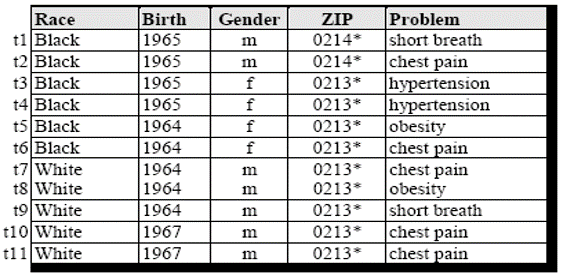
\includegraphics[width=100mm,scale=0.5]{Images/k2Diversified.png}
    \caption{A k=2, k-Anonymized Dataset. Source:\cite{sweeney2002k}}
    \label{fig:kAon=2}
\end{figure}

\paragraph{}
As apparent from the definition above, we need a very specialized database (where the values follow the rules for required k). If the complete database does not pass this test we can not publish it in full, instead we need to find a valid subset or add dummy (invalid) records to fulfill this requirement. Another way to achieve k-anonymity is to suppress (delete) some values (i.e. replace them by *, for example in the example above we suppressed the last digit of the zip code for the table to comply with 2-Anonymity definition) Finding valid subsets can be computationally very expensive so most often we suppress or just add dummy records. Adding invalid records or suppressing can also affect the quality of the data analysis that can be performed on the published set (as we may alter the original distribution of the data).
\paragraph{}
Another problem with this k-anonymity is that it fails if additional information is available to an adversary (who is looking to identify particular records). There are mainly two types of these attacks. First one is Homogeneity Attack, where using some previously known information adversary is able to filter out a set of records which have the same Secret Values (resulting in disclosure). For example if adversary knows that a person is Male, White and is 50 years old, he gets 2 matching records, both of them reveal secret value as `chest pain'. The other attack is known as Background Information Attack, where if an attacker is able to filter some data, the identification can be done by some general known information, for example, lets say white people are more prone to obesity. Countering such attacks have been proposed, by using l-diversity \cite{machanavajjhala2006diversity} which makes sure that each similar block of quasi-identifiers has at minimum l different sensitive values.

\paragraph{}
By its very nature, k-anonymity is limited to only pre-planned publishing of data, where the publisher has to keep the required k level of anonymity, valid for any values in the data. Any kind of interactive querying via this technique is not possible. But still there are some applications where k-anonymity has proven useful, as Intel demonstrated in it analysis of cloud usage data to enhance security \cite{sedayao2012enhancing}. 




\subsection{Privacy Preserving Data Mining Algorithms}
In one of the early works on privacy preservation, Privacy Preserving Data Mining Algorithms \cite{agrawal2001design} authors argue that data mining tasks usually don’t need individual records, but the distribution of data itself. If they perturbate the original distribution with some known random distribution, then they can infer the properties of original distribution by reconstructing it with confidence. This approach hides the individuals in distribution, thus allowing data analysis without privacy fears.
\paragraph{}
This technique is valid for offline data analysis where the data provider gives out all data at once (transformed into new distribution) to the analyzer, so applying it to real time data analysis where the analyzer might ask questions about data (like max of value Y, or sum of all Xs) is not possible.
\subsection{Differential Privacy}
Differential Privacy \cite{Dwork:2006:DP:2097282.2097284}, is a mathematically proven way to insure and quantify privacy. The main goal of this technique is to ensure that, no single record level information can be derived from the result of a computation done over the complete database of records. For example, such leaks can result from aggregation queries like Sum, Count and Min/Max, or where the database can be augmented with some auxiliary information. In this work, authors propose a mechanism to ensure the privacy condition, by adding controlled amount of random noise (usually from Laplacian Distribution) into the data or the results being produced.

There is usually a trade off between: the amount of noise and the utility of the results required. We will explore this technique in detail in the next chapter.


\subsection{Manual Data/Job Partitioning}
\paragraph{}
Some of the existing frameworks discussed in next section are based on manual division of data. This means that if an organization has both sensitive (private) and non-sensitive data, private data can be kept on local infrastructure and non-sensitive data can be given to public compute providers.
\paragraph{}
Approaches \cite{zhang2011sedic}\cite{xu2015framework} (c) and \cite{ko2011hybrex} (e) use this concept to apply analysis task on hybrid environment.
The drawback of this approach is that some human will have to decide and manually label the data, which will need human effort and extra cost.



\section{Existing Frameworks for Privacy Preserved Analysis}
\subsection{Privacy Integrated Queries}
\paragraph{}
Privacy Integrated Queries (PINQ) \cite{mcsherry2009privacy} build upon the idea of differential privacy by supplying an interface to standard LINQ queries in .NET. They try to offer non disclosing information by use of exponential noise and stable transforms. They demonstrate that their solution is also resistant to aggregation attacks, where the adversary may issue large number of queries, slightly varying in nature in an effort to combine results and getting to the underlying distribution.
\paragraph{}
One particular problem of this work regarding public cloud is this that PINQ requires a secure and trusted data store, as it’s an interface that transforms original data distribution to a new non disclosing distribution, that represents the original distribution. So this means, a complete public cloud implementation of this approach is not possible. This scenario, fits perfectly well with a hybrid model where storage is kept private and compute is delegated to public compute engines, however the data source must also provide the PINQ interface.
\subsection{Airavat}
\paragraph{}
Map Reduce is one of the most prevalent Big Data analysis tool, and Airavat \cite{roy2010airavat} modifies it to the task of privacy preservation. Here authors present a case where mappers are third party and hence their code is untrusted. It's methodology has two main components i.e. Mandated Access Control via the help of underlying operating system and application of differential privacy by adding random noise to the reduced outputs. For example, for the task of parallel K-Means clustering, mappers can be public which output cluster associations (within a bounded range) and the reducers can be private and trusted which output new cluster centroids with certain level of error, such that this error does not massively affect the collective distribution of points but also masks individual data points.
\paragraph{}
They applied their framework to multiple big data tasks like k-NN recommender engine, k Means clustering and Naïve Bayes Classifier and claim that their system has a performance overhead of 32\% (in terms of time complexity) compared to vanilla Map Reduce.
\paragraph{}
One problem with this performance score is this that the authors implemented this system entirely on public cloud i.e. 100 machine cluster on Amazon EC2, where most probably all machines were on same network, but in a hybrid environment such implementation will surely suffer performance loss because of added Virtual Network implementation (same problem as with HyberEx \cite{ko2011hybrex}).
\subsection{User labeled data protection}
\paragraph{}
Sedic \cite{zhang2011sedic} proposes an implementation of Map Reduce over Hybrid Cloud infrastructure. Their approach works by splitting up both the mappers and reducers over large number of nodes. They claim to preserve privacy by allowing the user to label critical data. They keep the sensitive data on private infrastructure and send out rest to public cloud.
\paragraph{}
[9] Also is similar to Sedic \cite{zhang2011sedic}, but they have proposed a mechanism to finely control the scale of tagging i.e. what is sensitive and what is not. They propose multi-level tagging in terms of: file level, line level, temporal and spatial level tags. This can give almost total control of information to an administrator but also adds the overhead of manual tagging effort.
\paragraph{}
Although both these approaches present a very good framework of task breakdown and scheduling but in terms of privacy, this approach is very simplistic and requires a lot of manual sanitization of data. Also as demonstrated by \cite{dwork2004privacy} this approach suffers from information leakage in presence of auxiliary information generator.
\subsection{GUPT: Privacy Preserving Data Analysis}
\paragraph{}
This framework \cite{mohan2012gupt} builds upon Airavat \cite{roy2010airavat} and presents two new concepts. First is Automatic Privacy Budget Allocations, authors argue that current data analysis experts have no idea about differential privacy hence they find it difficult to set privacy budgets i.e. the amount of noise in the output to obfuscate the sensitive information, even if they understand these concepts current tools and programs have to be redeveloped to comply with privacy guidelines. Hence they propose a mechanism to automatically allocate these privacy budgets and all other such parameters.
\paragraph{}
Secondly they propose the idea of decreased sensitivity of aged records, they give an example that very old records relating to deceased people, may not be as much privacy demanding as newer records. So they invest less resources hiding old information which gives them some performance improvements.
\subsection{HybrEx}
\paragraph{}
In this work \cite{ko2011hybrex} authors describe an execution strategy where they segregate both data and computation systems into trusted (private) and untrusted (public) partitions.
\paragraph{}
They manually label data as per the privacy requirements (safe to run publicly or not) and then use these labels to distribute the map and reduce jobs on hybrid environment. Private labeled data stays on private machines and public labeled data can be transferred to public cloud. The inherent nature of MapReduce requires all resources to be present in one network, so they used a Wide Area Network (WAN) encompassing cloud and private instances.
\paragraph{}
Authors realize that using a WAN impacts the performance of MapReduce jobs, but they claim that this performance hit is bearable. In this regard they compare the run-time of a job running on 5 local machines (937 sec) with 10 machine hybrid environment (702 sec).

\section{Comparison of the Available Frameworks}
\paragraph{}
All the mentioned frameworks use some form of manual data labeling, differential privacy or some combination of both. The table below summarizes these frameworks by describing their base fundamentals and their applicability to hybrid cloud environment:


\begin{table}[h]
\centering
\caption{Frameworks for privacy Oriented Analysis}
\label{Frameworks for privacy Oriented Analysis}
\resizebox{\textwidth}{!}{%
\begin{tabular}{|l|l|l|l|}
\hline
\textbf{Framework}                 & \textbf{Based on}    & \textbf{Hybrid Ready?} & \textbf{Accuracy} \\ \hline
Privacy Integrated Queries \cite{mcsherry2009privacy} & Differential Privacy & No                     &                   \\ \hline
Airavat \cite{roy2010airavat}                   & Differential Privacy & No                     &                   \\ \hline
Sedic \cite{zhang2011sedic} and Xu, X \cite{xu2015framework}    & Manual Labeling      & Yes                    &                   \\ \hline
GUPT \cite{mohan2012gupt}                      & Differential Privacy & No                     &                   \\ \hline
HybrEx \cite{ko2011hybrex}                    & Manual Labeling      & Yes                    &     Not Applicable              \\ \hline
\end{tabular}
}
\end{table}
\paragraph{}
It is apparent from the results above that, none of the existing techniques provides a comprehensive platform that uses differential privacy in a hybrid environment. This is important because in big data applications it becomes impractical to label data manually.
\paragraph{}
Note that nearly all of the frameworks, except Privacy Integrated Queries are based on MapReduce.
\paragraph{}
Also there is a need of specific use cases for privacy control, which can be used to compare all these approaches in a standard way. Currently privacy can mean a lot of different things for different people, like for a financial institute personal data of its customers (name and address) may not be as sensitive than their financial data (funds in accounts), but for a medical institute personal data is most sensitive. So in my further work I will try to demonstrate an actual real world use scenario.



\section{Chapter Conclusion}
\paragraph{}
Most of current frameworks for hybrid cloud, work by the manual tagging of sensitive information. Plus the standard mechanisms for differential privacy are hard for a data analyst, so there is scope of work in the direction of a unified framework that makes differential privacy techniques applicable in hybrid environment. 






\chapter{Location Based Services and Methodologies for Location Privacy}
\section{Location Based Services}
\paragraph{}
Today most of the mobile devices (phones, tablets, laptops etc.) have a GPS (Global Positioning System) receiver built in, it was not the case twenty years ago when this technology was limited to special professions, such as military and construction. The age of smart phones and mobile applications has unlocked a variety of useful applications of GPS. These services use location of the device or user to supply user with useful information. Such services are called Location Based Services (LBS).
\paragraph{}
LBS did exist before smartphones with GPS access, early LBS \cite{lbsShu} used mobile network positioning techniques like cellular triangulation. Although such services were useful but had a limited scope. Example of LBS from that era can be “Find my Friends” service which worked by a user sending a text message with his friends ID and the Network operator sending back the cell address (usually name of suburb) of the friend’s mobile (given that friend had previously agreed to his location sharing). Another example can be a SMS based restaurant locator, which would reply with a list of restaurants in the user’s vicinity. In this work however, we will focus mainly on the modern location services which have the ability to pinpoint a device's location to within a few meters \cite{ TGIS:TGIS1152}.
\paragraph{Examples of Location Based Services}
\begin{itemize}
\item Navigation (e.g Driving Directions)
\item Targeted Marketing (e.g. Sale/Offer near you!)
\item Nearby Point of Interest Discovery (e.g. Where is the nearest Chinese Restaurant?)
\item Information Services (e.g. Weather, News etc.)
\item Geo Targeted Content (e.g Online Radio may change content based on listener's location)
\end{itemize}

\subsection{Privacy Issues in Location Based Services}
All of these applications work by getting the location from the user's device and sending it to the server of the LBS provider. This sharing of location data raises some serious privacy issues. Exactly where a person is located is part of its human freedom, and most of the time, people will no want others to find where they are ``all the time". These others can be trusted entities (family or friends) or some adversarial entity (spies, robbers etc.). Yet most of us today transmit our location (via mobile phones) nearly 24/7, to servers we do not know about.

\paragraph{}
In a relatively early work \cite{dobson2003geoslavery} about the dangers of geo-privacy, authors have argued that location technologies that exist today, have the power to technically enslave human beings, for example they present scenarios where some ``master" entity may restrict the movement of ``slave" humans. Such an entity will have the technical means to accurately determine the location of slaves and take corrective action (just like we might zap animals with electric shock if they leave a set parameter). Although, such a scenario is very unlikely or even absurd, but authors argue that all the technological pre-requisites are available now, which itself is a cause of concern.

\paragraph{}
Mining of publicly available location data (such as: from social media) can have adverse affect on the privacy and even physical well being of the user. We have demonstrated such an experiment in Section ([Add Section]). 



\paragraph{}
Even if we do not go to such horrible extent, there will always be dangers in sharing and collecting location information. So the problem arises, that ``Can we extract any utility from LBSs, without compromising these privacy issues?". The answer is yes, there are multiple methodologies to analyze and process location data without exposing users to the risks of limiting freedom.  In the following sections we will explore some of these methods in detail.


\section{Methods for privacy aware Location Data Analysis}
\paragraph{}
There are many mechanisms for location privacy. Most of these approaches aim to limit the effect of any information that may be transmitted from a user's device. Nearly all the literature uses some kind of a motivation example as a use case for analysis.
\paragraph{A simple use scenario for LBS and desire for privacy:}

Figure \ref{fig:LBSMechanism} illustrates a simple use case of an LBS, which returns a list of restaurants (serving a specific cuisine), near a user's location. The general motivation of the Location Privacy Preserving approaches is to offer some utility, like list of Points of Interest (POI) (i.e. valid and geographically near restaurants Y,Z,A), while trying to hide as much of the original position X as possible. The alternate location that hides X is referred as location Z.
\begin{figure}[ht]
\centering
        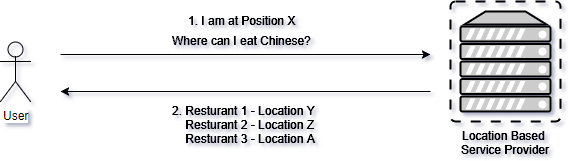
\includegraphics[width=100mm,scale=0.5]{Images/LBS-Scenario.png}
    \caption{LBS Mechanism}
    \label{fig:LBSMechanism}
\end{figure}

\paragraph{Definition of an adversary:}
Adversary in this setting, is any entity whose goal is to correctly intercept, calculate, determine or guess the location X of the user. Usually user would not give consent for this release of location to the adversary, hence its a breach of privacy.

\paragraph{Concept of Side Information}
Apart from ensuring privacy w.r.t location X some approaches also try to counter any prior knowledge any adversary might have, this prior information is also referred as side information in the literature. Notice that this side information can also be thought as (auxiliary information) when we talk about methods based on Differential Privacy. Side Information has the ability to render the obfuscation of location X useless. 


\paragraph{}
For example side information can be an actual map of the area where certain area is a water body i.e. pond, river etc. and if some Privacy Preserving technique outputs a location within this water body, an adversary can rule out this whole water area as possible location for the user. Another example can be that if adversary knows that a house has single bedroom and only one person lives there, he can infer when that house is empty based on social media usage pattern of that particular user (This is the exact experiment which we will demonstrate in section [Add Section]).

\subsection{Transformative Approaches}
There are some methods which transform the location information in such a way that the LBS can not infer location X but can provide some useful utility. One such method is \cite{khoshgozaran2007blind} which keeps encrypted POIs on server, they make sure that this encryption transformation supports Nearest Neighbour calculations. So user's device just transforms the actual location X by encrypting it using same mechanism and then LBS server calculate k-Nearest POIs and returns the list.

\paragraph{}
These type of approaches, are not very applicable today, as most of the information on all major LBS is in plain and not encrypted. This encryption at both server and client side can add a very substantial computing cost.



\subsection{Error Based Approaches}
\paragraph{}
Certain approaches work by minimizing the Expected Error between some obfuscated (the output) location and the actual full utility location, while constraining this error within some bound to maintain certain Quality of Service. \cite{shokri2012protecting} works by solving an optimization problem (via a linear program). The constraints they use for this linear program are: the expected quality of service and information taken from user's profile, so as to cancel out the effect of side information. To achieve this they present a game-theory based probabilistic model, where they counter any strategy that the adversary might use to win (guess actual location X). This work has a limitation, that you need to specify the type of side information, which may not be possible in a real world scenario. Other wise, if we limit the types of side information attacks in our model, this method yields the best quality of service (i.e. utility) among all such methods, but is computationally demanding because of solving linear program.



\paragraph{}
Another approach in this category \cite{hoh2005protecting}, works by adding noise to the paths user's take while moving, they aim to cross paths of different users, so as to confuse the adversary that which path belongs to which user, see Figure \ref{fig:pathConfusion}. The noise, or the perturbing factor can increase the chance of any two paths intersecting, which can effectively confuse the adversary. To calculate the best possible noisy intersecting paths (best: which confuse the most and still have acceptable Quality of Service) they also formulate an optimization problem like the previous approach. 
\begin{figure}[ht]
\centering
        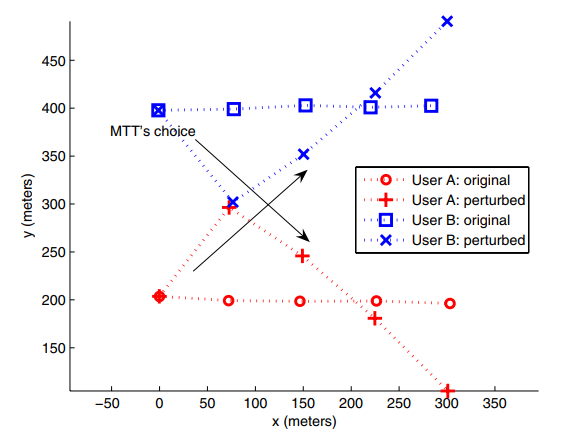
\includegraphics[width=75mm,scale=0.5]{Images/PathConfusion.PNG}
    \caption{Crossing two user's paths to confuse the adversary. Source:\cite{hoh2005protecting}}
    \label{fig:pathConfusion}
\end{figure}

\subsection{k-Anonymity and l-Diversity Based Approaches}
Some approaches have used to mask user's identity using making him indistinguishable with in k users, this is very similar to the approach we discussed in chapter 2.2.1 [Add Chapter]. Some interesting approaches like \cite{kido2005protection} work by reporting not the actual single location X to the LBS, but a set of multiple locations which contains X and all other values are dummy. Another approach \cite{duckham2005formal}, makes representative cloaking region around X and queries LBS on behalf of complete cloaking region. Figure \ref{fig:obfuscationRegion} shows basic idealization of this technique.


\begin{figure}[ht]
\centering
        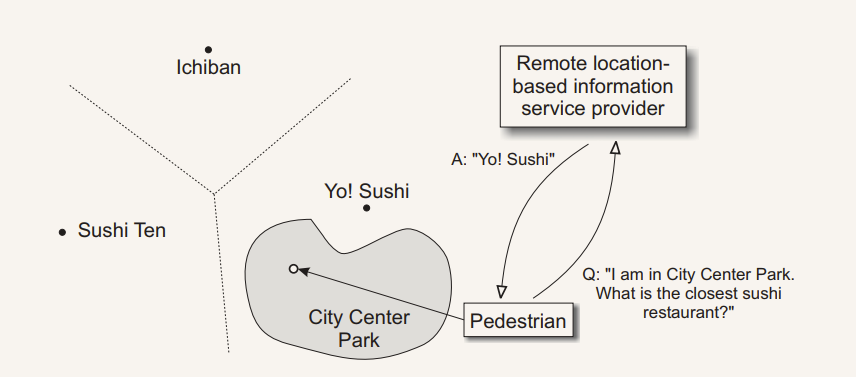
\includegraphics[width=120mm,scale=1]{Images/obfuscationRegion.PNG}
    \caption{Example of obfuscated cloaking region for pedestrian's location. Source:\cite{duckham2005formal}}
    \label{fig:obfuscationRegion}
\end{figure}

\paragraph{}
These approaches also suffers from side-information attack, as ensuring that all dummy locations are equally likely to be the real location X (from the point of view of the LBS) is hard to do. So the next set of approaches try to develop, a fit all model for location privacy, that abstract away the notion of side-information.



\subsection{Differential Privacy Based Approaches}
\paragraph{}
In Chapter 2 we introduced differential privacy as a method to do private data analysis, in this section we will discuss it specifically for location privacy. It is basically a balance between utility and a mathematical expression of privacy (we will offer detailed discussion on differential privacy in the next chapter).
\cite{dewri2013local} Proposes a framework where he makes up an anonymity set (similar to cloaking regions discussed earlier) having k locations and specifying the probability of reporting same location Z from this set to be similar (within a small range) for each of locations in the set. To achieve this similar probability distribution he adds Laplace noise to each location point in the set. One drawback of this technique is this that when he divides up the locations into sets, he kind of adds a deterministic element that can make the privacy guarantee weak. 
\paragraph{}
The seminal work on Location Privacy which can be termed as current state of the art is: Geo-Indistinguishability \cite{andres2013geo} introduced in 2012. This technique works by adding Laplacian Noise (drawn randomly form a specially constructed Planar Laplace distribution) to the actual location X to get a position Z (this is done offline i.e. on user's device). Now it sends Z to the LBS server and requests all the interesting service points with a set radius, called Area of Request (AOR). Ideally this radius being requested should be large enough that, it would contain X, as well as all the service points near X with in an Area of Interest (AOI) see Figure \ref{fig:AOIvsAOR}, that will offer best utility to the user. Now the device can easily filter AOI from AOR.
\begin{figure}[ht]
\centering
        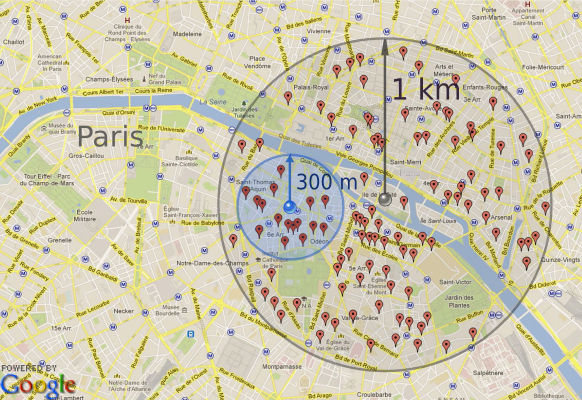
\includegraphics[width=100mm,scale=1]{Images/AOIvsAOR.PNG}
    \caption{AOI of 300m and AOR of 1 KM, X(blue) lies with in AOR. Source:\cite{andres2013geo}}
    \label{fig:AOIvsAOR}
\end{figure}

\paragraph{}
Note that, it is not guaranteed that  AOI and X will fall with in AOR, if this happens the scheme just considers such a request as not accepted. Authors state that if any attempt is made to dynamically set the radius of AOR, the LBS server would know that X lies with in that specific region. The uncertainty, that it is not guaranteed that X will be in AOR is the property that saves this approach from side information attacks, albeit at the cost of failed or unfulfilled requests where AOR does not include AOI.
\paragraph{}
One good advantage of this approach is that, it does not need a trusted middle layer to compute the obfuscated location Z, all can be done on user's device offline before sending Z to LBS.
\paragraph{Cloaking vs Planer-Laplace}
In \cite{andres2013geo} authors have presented a good comparison between the k-anonymity cloaking mechanism and their Planar Laplace method (explained above) see Figure \ref{fig:CloakingVsPlanar}. For this comparison they fixed the accuracy (i.e. utility) metric and compared the privacy metric on 3 different location maps a,b and c (having different point distributions). It is apparent that Planar Laplace gives better privacy guarantee, while abstracting the danger of side information attacks.

\begin{figure}[ht]
\centering
        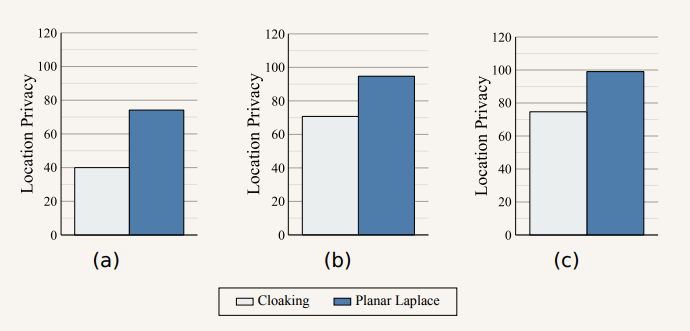
\includegraphics[width=120mm,scale=1]{Images/CloakingVsLaplace.PNG}
    \caption{Cloaking vs Planar Laplace at fixed utility. Source:\cite{andres2013geo}}
    \label{fig:CloakingVsPlanar}
\end{figure}


\section{Chapter Conclusion and A Possible Gap}
In this chapter we explained the mechanism of Location Based Services, and presented a survey of the current methods of ensuring privacy while working with LBSs. A lot of work has been done on the protection of user's location, but there are some very specific privacy related issues, that are concerned with the private properties/attributes of the locations themselves.For example: the use pattern of a house, people staying in a property, demographics of a apartment block. Although the goal of such analysis is not directly related to the techniques discussed in this chapter, but still its good to think about privacy issues for these applications. In chapter [Add Chapter] we will demonstrate, such an attack on privacy where we can infer when particular homes are empty, then we will propose a differential privacy based approach to extract some utility from this scenario.

\chapter{Differential Privacy}
\section{Introduction}
\paragraph{}
In Chapter 2 and 3, we introduced the notion of Differential Privacy with respect to a distributed environments and location privacy, In this chapter we will explore it in detail and formalize some of it's features. 

\paragraph{}
Differential Privacy \cite{Dwork:2006:DP:2097282.2097284} is one of the relatively new foundational works in preventing private information leaks. This work, first proves the impossibility of absolute disclosure prevention, which is the negation of Dalenius’s principal that no information should be learn-able from a data that is not learnable without absolute access to data. This auxiliary information is also dangerous for Privacy Preserving Data Mining Algorithms [2] as underlying distribution and some added information is usually sufficient to leak information.
\paragraph{}
To side step this impossibility authors propose a mechanism called differential privacy, which relaxes the absolute disclosure safety, that any information leak is within small multiplicative factor, i.e. adversary will at best have a rough approximation about the actual information. They achieve this by adding random noise to the output of queries. This magnitude of this noise is also controlled by the degree that one individual record can change the result of the query, for example getting mean of a distribution of small variance needs less noise but highly varying distributions require large amount of noise to conceal individual instances. \cite{dwork2014algorithmic} Provides a comprehensive analysis of differential privacy fundamentals and sets it in strong mathematical background. 
\paragraph{}
All these techniques have been proven to be effective only when the adversary tries sub linear number of queries, a large number of queries increase the chance of information leakage\cite{haeberlen2011differential}. \cite{dwork2004privacy} Argue that this limitation of sub-linear queries can be solved by using vertically partitioned databases, i.e. single attribute databases or database divided into multiple databases via subsets of attributes.
\paragraph{}
Differential Privacy seems to be the most trustworthy technique of all the approaches as its mathematically sound and provable. Other approaches need some form of trust between data provider and analyzer.
\paragraph{}
One problem with differential privacy is this that currently there are no standard ways to do this, like RSA or AES are now standard implementations of Public Key Encryption and have made encryption adoptable and more secure. So I believe that, such a standard will really help Differential Privacy to be adopted on a large scale.



\newcommand{\dd}[1]{\mathrm{d}#1}

\begin{equation}
[Pr[\mathit{K}(D_{1})\in S] \leq \exp (\epsilon ) \times Pr[\mathit{K}(D_{2})\in S]] \end{equation}

\begin{equation}
[Pr[\mathit{K}(D_{1})\in S]  = Pr[\mathit{K}(D_{2})\in S]]
\end{equation}


\chapter{Experimental Setup - Apache Hadoop and Spark on NECTAR}




\chapter{Location Privacy and Attack Demo }

\chapter{Location Specific Privacy Attack and Resolution}




\chapter{Conclusion and Recommendations}


\bibliographystyle{plain}
\bibliography{references}
\end{document}
